\documentclass[1p]{elsarticle_modified}
%\bibliographystyle{elsarticle-num}

%\usepackage[colorlinks]{hyperref}
%\usepackage{abbrmath_seonhwa} %\Abb, \Ascr, \Acal ,\Abf, \Afrak
\usepackage{amsfonts}
\usepackage{amssymb}
\usepackage{amsmath}
\usepackage{amsthm}
\usepackage{scalefnt}
\usepackage{amsbsy}
\usepackage{kotex}
\usepackage{caption}
\usepackage{subfig}
\usepackage{color}
\usepackage{graphicx}
\usepackage{xcolor} %% white, black, red, green, blue, cyan, magenta, yellow
\usepackage{float}
\usepackage{setspace}
\usepackage{hyperref}

\usepackage{tikz}
\usetikzlibrary{arrows}

\usepackage{multirow}
\usepackage{array} % fixed length table
\usepackage{hhline}

%%%%%%%%%%%%%%%%%%%%%
\makeatletter
\renewcommand*\env@matrix[1][\arraystretch]{%
	\edef\arraystretch{#1}%
	\hskip -\arraycolsep
	\let\@ifnextchar\new@ifnextchar
	\array{*\c@MaxMatrixCols c}}
\makeatother %https://tex.stackexchange.com/questions/14071/how-can-i-increase-the-line-spacing-in-a-matrix
%%%%%%%%%%%%%%%

\usepackage[normalem]{ulem}

\newcommand{\msout}[1]{\ifmmode\text{\sout{\ensuremath{#1}}}\else\sout{#1}\fi}
%SOURCE: \msout is \stkout macro in https://tex.stackexchange.com/questions/20609/strikeout-in-math-mode

\newcommand{\cancel}[1]{
	\ifmmode
	{\color{red}\msout{#1}}
	\else
	{\color{red}\sout{#1}}
	\fi
}

\newcommand{\add}[1]{
	{\color{blue}\uwave{#1}}
}

\newcommand{\replace}[2]{
	\ifmmode
	{\color{red}\msout{#1}}{\color{blue}\uwave{#2}}
	\else
	{\color{red}\sout{#1}}{\color{blue}\uwave{#2}}
	\fi
}

\newcommand{\Sol}{\mathcal{S}} %segment
\newcommand{\D}{D} %diagram
\newcommand{\A}{\mathcal{A}} %arc


%%%%%%%%%%%%%%%%%%%%%%%%%%%%%5 test

\def\sl{\operatorname{\textup{SL}}(2,\Cbb)}
\def\psl{\operatorname{\textup{PSL}}(2,\Cbb)}
\def\quan{\mkern 1mu \triangleright \mkern 1mu}

\theoremstyle{definition}
\newtheorem{thm}{Theorem}[section]
\newtheorem{prop}[thm]{Proposition}
\newtheorem{lem}[thm]{Lemma}
\newtheorem{ques}[thm]{Question}
\newtheorem{cor}[thm]{Corollary}
\newtheorem{defn}[thm]{Definition}
\newtheorem{exam}[thm]{Example}
\newtheorem{rmk}[thm]{Remark}
\newtheorem{alg}[thm]{Algorithm}

\newcommand{\I}{\sqrt{-1}}
\begin{document}

%\begin{frontmatter}
%
%\title{Boundary parabolic representations of knots up to 8 crossings}
%
%%% Group authors per affiliation:
%\author{Yunhi Cho} 
%\address{Department of Mathematics, University of Seoul, Seoul, Korea}
%\ead{yhcho@uos.ac.kr}
%
%
%\author{Seonhwa Kim} %\fnref{s_kim}}
%\address{Center for Geometry and Physics, Institute for Basic Science, Pohang, 37673, Korea}
%\ead{ryeona17@ibs.re.kr}
%
%\author{Hyuk Kim}
%\address{Department of Mathematical Sciences, Seoul National University, Seoul 08826, Korea}
%\ead{hyukkim@snu.ac.kr}
%
%\author{Seokbeom Yoon}
%\address{Department of Mathematical Sciences, Seoul National University, Seoul, 08826,  Korea}
%\ead{sbyoon15@snu.ac.kr}
%
%\begin{abstract}
%We find all boundary parabolic representation of knots up to 8 crossings.
%
%\end{abstract}
%\begin{keyword}
%    \MSC[2010] 57M25 
%\end{keyword}
%
%\end{frontmatter}

%\linenumbers
%\tableofcontents
%
\newcommand\colored[1]{\textcolor{white}{\rule[-0.35ex]{0.8em}{1.4ex}}\kern-0.8em\color{red} #1}%
%\newcommand\colored[1]{\textcolor{white}{ #1}\kern-2.17ex	\textcolor{white}{ #1}\kern-1.81ex	\textcolor{white}{ #1}\kern-2.15ex\color{red}#1	}

{\Large $\underline{12a_{0034}~(K12a_{0034})}$}

\setlength{\tabcolsep}{10pt}
\renewcommand{\arraystretch}{1.6}
\vspace{1cm}\begin{tabular}{m{100pt}>{\centering\arraybackslash}m{274pt}}
\multirow{5}{120pt}{
	\centering
	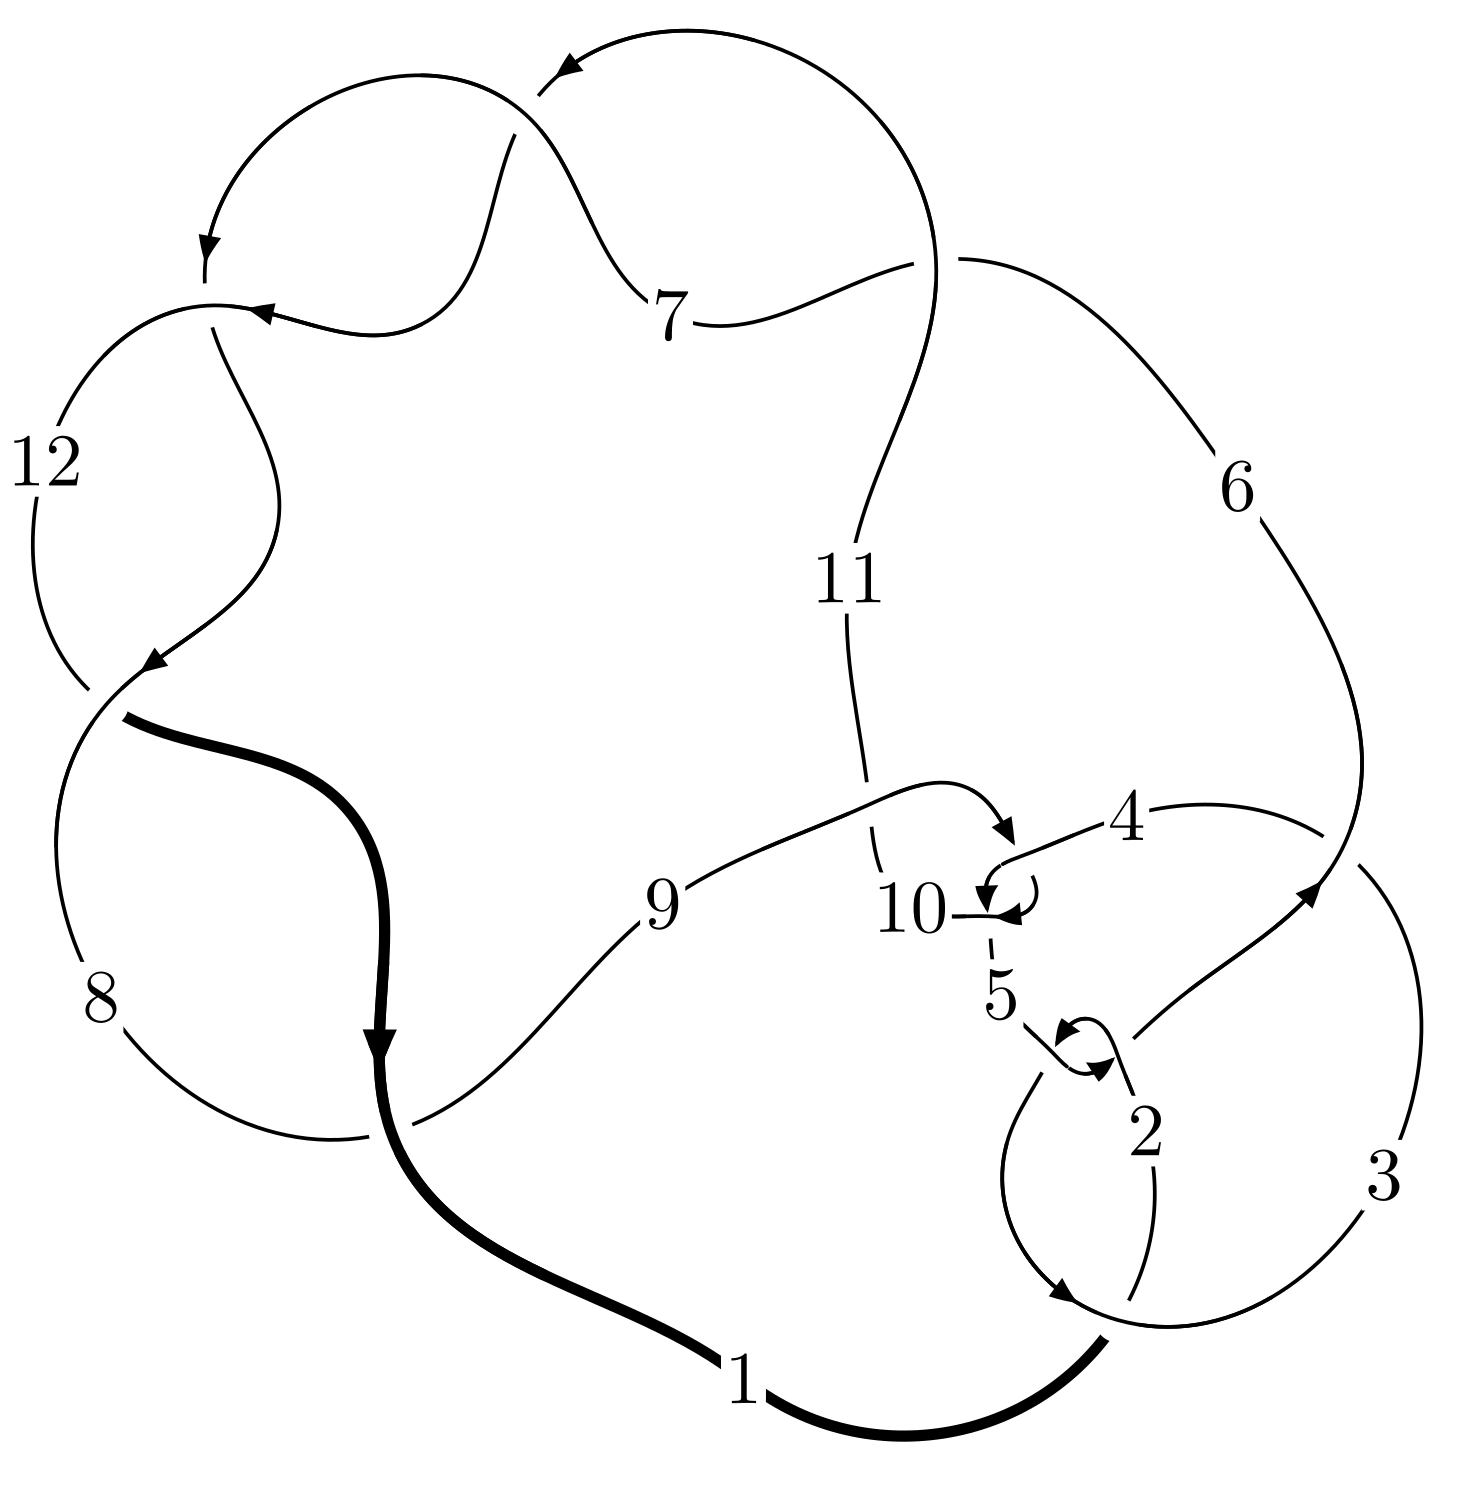
\includegraphics[width=112pt]{../../../GIT/diagram.site/Diagrams/png/835_12a_0034.png}\\
\ \ \ A knot diagram\footnotemark}&
\allowdisplaybreaks
\textbf{Linearized knot diagam} \\
\cline{2-2}
 &
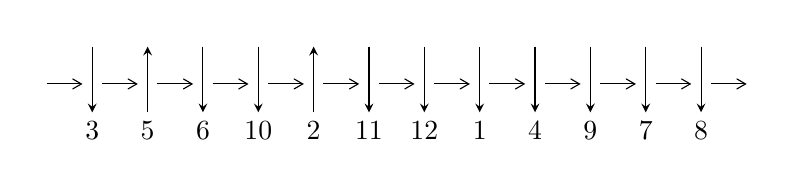
\begin{tikzpicture}[x=20pt, y=17pt]
	% nodes
	\node (C0) at (0, 0) {};
	\node (C1) at (1, 0) {};
	\node (C1U) at (1, +1) {};
	\node (C1D) at (1, -1) {3};

	\node (C2) at (2, 0) {};
	\node (C2U) at (2, +1) {};
	\node (C2D) at (2, -1) {5};

	\node (C3) at (3, 0) {};
	\node (C3U) at (3, +1) {};
	\node (C3D) at (3, -1) {6};

	\node (C4) at (4, 0) {};
	\node (C4U) at (4, +1) {};
	\node (C4D) at (4, -1) {10};

	\node (C5) at (5, 0) {};
	\node (C5U) at (5, +1) {};
	\node (C5D) at (5, -1) {2};

	\node (C6) at (6, 0) {};
	\node (C6U) at (6, +1) {};
	\node (C6D) at (6, -1) {11};

	\node (C7) at (7, 0) {};
	\node (C7U) at (7, +1) {};
	\node (C7D) at (7, -1) {12};

	\node (C8) at (8, 0) {};
	\node (C8U) at (8, +1) {};
	\node (C8D) at (8, -1) {1};

	\node (C9) at (9, 0) {};
	\node (C9U) at (9, +1) {};
	\node (C9D) at (9, -1) {4};

	\node (C10) at (10, 0) {};
	\node (C10U) at (10, +1) {};
	\node (C10D) at (10, -1) {9};

	\node (C11) at (11, 0) {};
	\node (C11U) at (11, +1) {};
	\node (C11D) at (11, -1) {7};

	\node (C12) at (12, 0) {};
	\node (C12U) at (12, +1) {};
	\node (C12D) at (12, -1) {8};
	\node (C13) at (13, 0) {};

	% arrows
	\draw[->,>={angle 60}]
	(C0) edge (C1) (C1) edge (C2) (C2) edge (C3) (C3) edge (C4) (C4) edge (C5) (C5) edge (C6) (C6) edge (C7) (C7) edge (C8) (C8) edge (C9) (C9) edge (C10) (C10) edge (C11) (C11) edge (C12) (C12) edge (C13) ;	\draw[->,>=stealth]
	(C1U) edge (C1D) (C2D) edge (C2U) (C3U) edge (C3D) (C4U) edge (C4D) (C5D) edge (C5U) (C6U) edge (C6D) (C7U) edge (C7D) (C8U) edge (C8D) (C9U) edge (C9D) (C10U) edge (C10D) (C11U) edge (C11D) (C12U) edge (C12D) ;
	\end{tikzpicture} \\
\hhline{~~} \\& 
\textbf{Solving Sequence} \\ \cline{2-2} 
 &
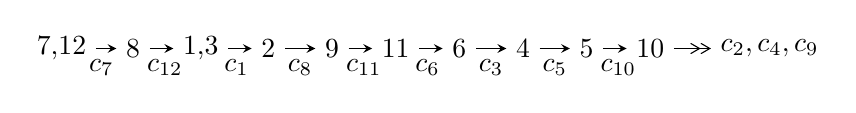
\begin{tikzpicture}[x=23pt, y=7pt]
	% node
	\node (A0) at (-1/8, 0) {7,12};
	\node (A1) at (1, 0) {8};
	\node (A2) at (33/16, 0) {1,3};
	\node (A3) at (25/8, 0) {2};
	\node (A4) at (33/8, 0) {9};
	\node (A5) at (41/8, 0) {11};
	\node (A6) at (49/8, 0) {6};
	\node (A7) at (57/8, 0) {4};
	\node (A8) at (65/8, 0) {5};
	\node (A9) at (73/8, 0) {10};
	\node (C1) at (1/2, -1) {$c_{7}$};
	\node (C2) at (3/2, -1) {$c_{12}$};
	\node (C3) at (21/8, -1) {$c_{1}$};
	\node (C4) at (29/8, -1) {$c_{8}$};
	\node (C5) at (37/8, -1) {$c_{11}$};
	\node (C6) at (45/8, -1) {$c_{6}$};
	\node (C7) at (53/8, -1) {$c_{3}$};
	\node (C8) at (61/8, -1) {$c_{5}$};
	\node (C9) at (69/8, -1) {$c_{10}$};
	\node (A10) at (11, 0) {$c_{2},c_{4},c_{9}$};

	% edge
	\draw[->,>=stealth]	
	(A0) edge (A1) (A1) edge (A2) (A2) edge (A3) (A3) edge (A4) (A4) edge (A5) (A5) edge (A6) (A6) edge (A7) (A7) edge (A8) (A8) edge (A9) ;
	\draw[->>,>={angle 60}]	
	(A9) edge (A10);
\end{tikzpicture} \\ 

\end{tabular} \\

\footnotetext{
The image of knot diagram is generated by the software ``\textbf{Draw programme}" developed by Andrew Bartholomew(\url{http://www.layer8.co.uk/maths/draw/index.htm\#Running-draw}), where we modified some parts for our purpose(\url{https://github.com/CATsTAILs/LinksPainter}).
}\phantom \\ \newline 
\centering \textbf{Ideals for irreducible components\footnotemark of $X_{\text{par}}$} 
 
\begin{align*}
I^u_{1}&=\langle 
-11 u^{60}+15 u^{59}+\cdots+2 b+7,\;-8 u^{60}+9 u^{59}+\cdots+2 a+7,\;u^{61}-3 u^{60}+\cdots+u+1\rangle \\
I^u_{2}&=\langle 
a u+b- a,\;a^2+a u+a+u+2,\;u^2+u-1\rangle \\
\\
\end{align*}
\raggedright * 2 irreducible components of $\dim_{\mathbb{C}}=0$, with total 65 representations.\\
\footnotetext{All coefficients of polynomials are rational numbers. But the coefficients are sometimes approximated in decimal forms when there is not enough margin.}
\newpage
\renewcommand{\arraystretch}{1}
\centering \section*{I. $I^u_{1}= \langle -11 u^{60}+15 u^{59}+\cdots+2 b+7,\;-8 u^{60}+9 u^{59}+\cdots+2 a+7,\;u^{61}-3 u^{60}+\cdots+u+1 \rangle$}
\flushleft \textbf{(i) Arc colorings}\\
\begin{tabular}{m{7pt} m{180pt} m{7pt} m{180pt} }
\flushright $a_{7}=$&$\begin{pmatrix}1\\0\end{pmatrix}$ \\
\flushright $a_{12}=$&$\begin{pmatrix}0\\u\end{pmatrix}$ \\
\flushright $a_{8}=$&$\begin{pmatrix}1\\u^2\end{pmatrix}$ \\
\flushright $a_{1}=$&$\begin{pmatrix}- u\\- u^3+u\end{pmatrix}$ \\
\flushright $a_{3}=$&$\begin{pmatrix}4 u^{60}-\frac{9}{2} u^{59}+\cdots-6 u-\frac{7}{2}\\\frac{11}{2} u^{60}-\frac{15}{2} u^{59}+\cdots-\frac{11}{2} u-\frac{7}{2}\end{pmatrix}$ \\
\flushright $a_{2}=$&$\begin{pmatrix}-\frac{1}{2} u^{59}+u^{58}+\cdots+6 u-\frac{1}{2}\\-\frac{1}{2} u^{60}+\frac{1}{2} u^{59}+\cdots+\frac{5}{2} u+\frac{1}{2}\end{pmatrix}$ \\
\flushright $a_{9}=$&$\begin{pmatrix}- u^2+1\\- u^4+2 u^2\end{pmatrix}$ \\
\flushright $a_{11}=$&$\begin{pmatrix}u\\u\end{pmatrix}$ \\
\flushright $a_{6}=$&$\begin{pmatrix}- u^2+1\\- u^2\end{pmatrix}$ \\
\flushright $a_{4}=$&$\begin{pmatrix}\frac{19}{2} u^{60}-12 u^{59}+\cdots-\frac{21}{2} u-6\\\frac{27}{2} u^{60}-18 u^{59}+\cdots-\frac{25}{2} u-8\end{pmatrix}$ \\
\flushright $a_{5}=$&$\begin{pmatrix}-\frac{7}{2} u^{60}+5 u^{59}+\cdots+\frac{5}{2} u+2\\-\frac{15}{2} u^{60}+10 u^{59}+\cdots+\frac{15}{2} u+4\end{pmatrix}$ \\
\flushright $a_{10}=$&$\begin{pmatrix}- u^7+4 u^5-4 u^3+2 u\\- u^9+5 u^7-7 u^5+2 u^3+u\end{pmatrix}$\\&\end{tabular}
\flushleft \textbf{(ii) Obstruction class $= -1$}\\~\\
\flushleft \textbf{(iii) Cusp Shapes $= -\frac{5}{2} u^{60}+95 u^{58}+\cdots-\frac{29}{2} u-5$}\\~\\
\newpage\renewcommand{\arraystretch}{1}
\flushleft \textbf{(iv) u-Polynomials at the component}\newline \\
\begin{tabular}{m{50pt}|m{274pt}}
Crossings & \hspace{64pt}u-Polynomials at each crossing \\
\hline $$\begin{aligned}c_{1}\end{aligned}$$&$\begin{aligned}
&u^{61}+29 u^{60}+\cdots+23 u-1
\end{aligned}$\\
\hline $$\begin{aligned}c_{2},c_{5}\end{aligned}$$&$\begin{aligned}
&u^{61}+3 u^{60}+\cdots+9 u+1
\end{aligned}$\\
\hline $$\begin{aligned}c_{3}\end{aligned}$$&$\begin{aligned}
&u^{61}-3 u^{60}+\cdots-129 u+241
\end{aligned}$\\
\hline $$\begin{aligned}c_{4},c_{9}\end{aligned}$$&$\begin{aligned}
&u^{61}+u^{60}+\cdots-48 u-16
\end{aligned}$\\
\hline $$\begin{aligned}c_{6},c_{7},c_{8}\\c_{11},c_{12}\end{aligned}$$&$\begin{aligned}
&u^{61}+3 u^{60}+\cdots+u-1
\end{aligned}$\\
\hline $$\begin{aligned}c_{10}\end{aligned}$$&$\begin{aligned}
&u^{61}+25 u^{60}+\cdots+2432 u+256
\end{aligned}$\\
\hline
\end{tabular}\\~\\
\newpage\renewcommand{\arraystretch}{1}
\flushleft \textbf{(v) Riley Polynomials at the component}\newline \\
\begin{tabular}{m{50pt}|m{274pt}}
Crossings & \hspace{64pt}Riley Polynomials at each crossing \\
\hline $$\begin{aligned}c_{1}\end{aligned}$$&$\begin{aligned}
&y^{61}+9 y^{60}+\cdots+707 y-1
\end{aligned}$\\
\hline $$\begin{aligned}c_{2},c_{5}\end{aligned}$$&$\begin{aligned}
&y^{61}+29 y^{60}+\cdots+23 y-1
\end{aligned}$\\
\hline $$\begin{aligned}c_{3}\end{aligned}$$&$\begin{aligned}
&y^{61}-11 y^{60}+\cdots+2638239 y-58081
\end{aligned}$\\
\hline $$\begin{aligned}c_{4},c_{9}\end{aligned}$$&$\begin{aligned}
&y^{61}-25 y^{60}+\cdots+2432 y-256
\end{aligned}$\\
\hline $$\begin{aligned}c_{6},c_{7},c_{8}\\c_{11},c_{12}\end{aligned}$$&$\begin{aligned}
&y^{61}-79 y^{60}+\cdots+19 y-1
\end{aligned}$\\
\hline $$\begin{aligned}c_{10}\end{aligned}$$&$\begin{aligned}
&y^{61}+15 y^{60}+\cdots+2564096 y-65536
\end{aligned}$\\
\hline
\end{tabular}\\~\\
\newpage\flushleft \textbf{(vi) Complex Volumes and Cusp Shapes}
$$\begin{array}{c|c|c}  
\text{Solutions to }I^u_{1}& \I (\text{vol} + \sqrt{-1}CS) & \text{Cusp shape}\\
 \hline 
\begin{aligned}
u &= -0.941549 + 0.362904 I \\
a &= -0.926027 - 0.288989 I \\
b &= \phantom{-}0.684803 + 0.361766 I\end{aligned}
 & -1.57693 + 6.68347 I & \phantom{-0.000000 } 0 \\ \hline\begin{aligned}
u &= -0.941549 - 0.362904 I \\
a &= -0.926027 + 0.288989 I \\
b &= \phantom{-}0.684803 - 0.361766 I\end{aligned}
 & -1.57693 - 6.68347 I & \phantom{-0.000000 } 0 \\ \hline\begin{aligned}
u &= -0.962161 + 0.388897 I \\
a &= \phantom{-}1.091940 + 0.880454 I \\
b &= -0.891980 - 0.179165 I\end{aligned}
 & -3.85828 + 11.82190 I & \phantom{-0.000000 } 0 \\ \hline\begin{aligned}
u &= -0.962161 - 0.388897 I \\
a &= \phantom{-}1.091940 - 0.880454 I \\
b &= -0.891980 + 0.179165 I\end{aligned}
 & -3.85828 - 11.82190 I & \phantom{-0.000000 } 0 \\ \hline\begin{aligned}
u &= -0.991302 + 0.313503 I \\
a &= -0.066752 + 0.371102 I \\
b &= -0.789116 - 0.780549 I\end{aligned}
 & -6.39349 + 4.01306 I & \phantom{-0.000000 } 0 \\ \hline\begin{aligned}
u &= -0.991302 - 0.313503 I \\
a &= -0.066752 - 0.371102 I \\
b &= -0.789116 + 0.780549 I\end{aligned}
 & -6.39349 - 4.01306 I & \phantom{-0.000000 } 0 \\ \hline\begin{aligned}
u &= \phantom{-}0.907581 + 0.284646 I \\
a &= -1.43188 + 0.77881 I \\
b &= \phantom{-}1.194390 - 0.037845 I\end{aligned}
 & -1.92448 - 5.85744 I & \phantom{-0.000000 } 0 \\ \hline\begin{aligned}
u &= \phantom{-}0.907581 - 0.284646 I \\
a &= -1.43188 - 0.77881 I \\
b &= \phantom{-}1.194390 + 0.037845 I\end{aligned}
 & -1.92448 + 5.85744 I & \phantom{-0.000000 } 0 \\ \hline\begin{aligned}
u &= -1.06207\phantom{ +0.000000I} \\
a &= -0.867883\phantom{ +0.000000I} \\
b &= \phantom{-}0.339270\phantom{ +0.000000I}\end{aligned}
 & -5.58398\phantom{ +0.000000I} & \phantom{-0.000000 } 0 \\ \hline\begin{aligned}
u &= \phantom{-}0.916155 + 0.124387 I \\
a &= -0.395310 + 0.861467 I \\
b &= \phantom{-}0.790911 - 1.053260 I\end{aligned}
 & -3.56819 + 0.84716 I & -15.9906 + 0. I\phantom{ +0.000000I}\\
 \hline 
 \end{array}$$\newpage$$\begin{array}{c|c|c}  
\text{Solutions to }I^u_{1}& \I (\text{vol} + \sqrt{-1}CS) & \text{Cusp shape}\\
 \hline 
\begin{aligned}
u &= \phantom{-}0.916155 - 0.124387 I \\
a &= -0.395310 - 0.861467 I \\
b &= \phantom{-}0.790911 + 1.053260 I\end{aligned}
 & -3.56819 - 0.84716 I & -15.9906 + 0. I\phantom{ +0.000000I} \\ \hline\begin{aligned}
u &= -0.858548 + 0.285771 I \\
a &= -0.240294 + 1.130700 I \\
b &= \phantom{-}0.426613 + 0.684373 I\end{aligned}
 & -0.14613 + 4.14771 I & -8.00000 - 7.53022 I \\ \hline\begin{aligned}
u &= -0.858548 - 0.285771 I \\
a &= -0.240294 - 1.130700 I \\
b &= \phantom{-}0.426613 - 0.684373 I\end{aligned}
 & -0.14613 - 4.14771 I & -8.00000 + 7.53022 I \\ \hline\begin{aligned}
u &= \phantom{-}0.833612 + 0.279640 I \\
a &= \phantom{-}1.133180 - 0.204262 I \\
b &= -0.769914 + 0.142240 I\end{aligned}
 & \phantom{-}0.014847 - 1.230250 I & -8.00000 + 2.00002 I \\ \hline\begin{aligned}
u &= \phantom{-}0.833612 - 0.279640 I \\
a &= \phantom{-}1.133180 + 0.204262 I \\
b &= -0.769914 - 0.142240 I\end{aligned}
 & \phantom{-}0.014847 + 1.230250 I & -8.00000 - 2.00002 I \\ \hline\begin{aligned}
u &= -1.138410 + 0.086480 I \\
a &= \phantom{-}0.760786 + 0.178531 I \\
b &= -0.780459 + 0.648714 I\end{aligned}
 & -8.82704 + 3.92280 I & \phantom{-0.000000 } 0 \\ \hline\begin{aligned}
u &= -1.138410 - 0.086480 I \\
a &= \phantom{-}0.760786 - 0.178531 I \\
b &= -0.780459 - 0.648714 I\end{aligned}
 & -8.82704 - 3.92280 I & \phantom{-0.000000 } 0 \\ \hline\begin{aligned}
u &= -0.819047 + 0.217033 I \\
a &= -0.57338 - 1.48189 I \\
b &= -0.544215 - 0.744173 I\end{aligned}
 & -1.09072 - 0.91618 I & -13.20392 - 2.90788 I \\ \hline\begin{aligned}
u &= -0.819047 - 0.217033 I \\
a &= -0.57338 + 1.48189 I \\
b &= -0.544215 + 0.744173 I\end{aligned}
 & -1.09072 + 0.91618 I & -13.20392 + 2.90788 I \\ \hline\begin{aligned}
u &= \phantom{-}0.651545 + 0.456443 I \\
a &= \phantom{-}0.43685 - 1.47583 I \\
b &= \phantom{-}0.607385 - 0.419645 I\end{aligned}
 & -2.01345 + 4.76879 I & -12.80458 - 3.25405 I\\
 \hline 
 \end{array}$$\newpage$$\begin{array}{c|c|c}  
\text{Solutions to }I^u_{1}& \I (\text{vol} + \sqrt{-1}CS) & \text{Cusp shape}\\
 \hline 
\begin{aligned}
u &= \phantom{-}0.651545 - 0.456443 I \\
a &= \phantom{-}0.43685 + 1.47583 I \\
b &= \phantom{-}0.607385 + 0.419645 I\end{aligned}
 & -2.01345 - 4.76879 I & -12.80458 + 3.25405 I \\ \hline\begin{aligned}
u &= \phantom{-}0.672132 + 0.371659 I \\
a &= \phantom{-}0.204778 + 0.807835 I \\
b &= -0.503235 + 0.231907 I\end{aligned}
 & \phantom{-}0.006977 + 0.191932 I & -9.14973 + 0.93355 I \\ \hline\begin{aligned}
u &= \phantom{-}0.672132 - 0.371659 I \\
a &= \phantom{-}0.204778 - 0.807835 I \\
b &= -0.503235 - 0.231907 I\end{aligned}
 & \phantom{-}0.006977 - 0.191932 I & -9.14973 - 0.93355 I \\ \hline\begin{aligned}
u &= \phantom{-}0.486313 + 0.449825 I \\
a &= \phantom{-}1.064050 + 0.128423 I \\
b &= \phantom{-}0.750517 + 0.088709 I\end{aligned}
 & -3.44842 - 2.18500 I & -15.5614 + 4.6731 I \\ \hline\begin{aligned}
u &= \phantom{-}0.486313 - 0.449825 I \\
a &= \phantom{-}1.064050 - 0.128423 I \\
b &= \phantom{-}0.750517 - 0.088709 I\end{aligned}
 & -3.44842 + 2.18500 I & -15.5614 - 4.6731 I \\ \hline\begin{aligned}
u &= \phantom{-}0.142006 + 0.624563 I \\
a &= \phantom{-}0.949731 - 0.841604 I \\
b &= \phantom{-}1.063740 + 0.386697 I\end{aligned}
 & -0.47167 - 8.39775 I & -9.16009 + 8.05408 I \\ \hline\begin{aligned}
u &= \phantom{-}0.142006 - 0.624563 I \\
a &= \phantom{-}0.949731 + 0.841604 I \\
b &= \phantom{-}1.063740 - 0.386697 I\end{aligned}
 & -0.47167 + 8.39775 I & -9.16009 - 8.05408 I \\ \hline\begin{aligned}
u &= \phantom{-}0.119463 + 0.584881 I \\
a &= -0.402048 + 0.694739 I \\
b &= -0.574572 - 0.527063 I\end{aligned}
 & \phantom{-}1.67223 - 3.47107 I & -5.43201 + 4.12123 I \\ \hline\begin{aligned}
u &= \phantom{-}0.119463 - 0.584881 I \\
a &= -0.402048 - 0.694739 I \\
b &= -0.574572 + 0.527063 I\end{aligned}
 & \phantom{-}1.67223 + 3.47107 I & -5.43201 - 4.12123 I \\ \hline\begin{aligned}
u &= \phantom{-}0.222473 + 0.540240 I \\
a &= \phantom{-}0.01204 - 1.43662 I \\
b &= \phantom{-}0.230433 - 0.262534 I\end{aligned}
 & -2.65865 - 1.12584 I & -12.84225 + 3.10905 I\\
 \hline 
 \end{array}$$\newpage$$\begin{array}{c|c|c}  
\text{Solutions to }I^u_{1}& \I (\text{vol} + \sqrt{-1}CS) & \text{Cusp shape}\\
 \hline 
\begin{aligned}
u &= \phantom{-}0.222473 - 0.540240 I \\
a &= \phantom{-}0.01204 + 1.43662 I \\
b &= \phantom{-}0.230433 + 0.262534 I\end{aligned}
 & -2.65865 + 1.12584 I & -12.84225 - 3.10905 I \\ \hline\begin{aligned}
u &= \phantom{-}0.011799 + 0.502580 I \\
a &= \phantom{-}0.736143 + 0.780204 I \\
b &= \phantom{-}0.443073 - 0.686495 I\end{aligned}
 & \phantom{-}2.47447 - 1.45390 I & -2.95032 + 3.27697 I \\ \hline\begin{aligned}
u &= \phantom{-}0.011799 - 0.502580 I \\
a &= \phantom{-}0.736143 - 0.780204 I \\
b &= \phantom{-}0.443073 + 0.686495 I\end{aligned}
 & \phantom{-}2.47447 + 1.45390 I & -2.95032 - 3.27697 I \\ \hline\begin{aligned}
u &= -0.071181 + 0.471890 I \\
a &= -1.39302 - 1.27147 I \\
b &= -0.971413 + 0.506703 I\end{aligned}
 & \phantom{-}1.06320 + 3.26175 I & -5.16927 - 3.30010 I \\ \hline\begin{aligned}
u &= -0.071181 - 0.471890 I \\
a &= -1.39302 + 1.27147 I \\
b &= -0.971413 - 0.506703 I\end{aligned}
 & \phantom{-}1.06320 - 3.26175 I & -5.16927 + 3.30010 I \\ \hline\begin{aligned}
u &= \phantom{-}0.441573\phantom{ +0.000000I} \\
a &= \phantom{-}0.291655\phantom{ +0.000000I} \\
b &= -0.318830\phantom{ +0.000000I}\end{aligned}
 & -0.703516\phantom{ +0.000000I} & -13.9150\phantom{ +0.000000I} \\ \hline\begin{aligned}
u &= -1.57089 + 0.05487 I \\
a &= -0.108181 - 0.454338 I \\
b &= -0.73199 - 1.31069 I\end{aligned}
 & -9.35339 - 3.05356 I & \phantom{-0.000000 } 0 \\ \hline\begin{aligned}
u &= -1.57089 - 0.05487 I \\
a &= -0.108181 + 0.454338 I \\
b &= -0.73199 + 1.31069 I\end{aligned}
 & -9.35339 + 3.05356 I & \phantom{-0.000000 } 0 \\ \hline\begin{aligned}
u &= -1.62164 + 0.05572 I \\
a &= -0.661023 + 0.422089 I \\
b &= -1.01599 + 1.16132 I\end{aligned}
 & -7.88099 + 1.12428 I & \phantom{-0.000000 } 0 \\ \hline\begin{aligned}
u &= -1.62164 - 0.05572 I \\
a &= -0.661023 - 0.422089 I \\
b &= -1.01599 - 1.16132 I\end{aligned}
 & -7.88099 - 1.12428 I & \phantom{-0.000000 } 0\\
 \hline 
 \end{array}$$\newpage$$\begin{array}{c|c|c}  
\text{Solutions to }I^u_{1}& \I (\text{vol} + \sqrt{-1}CS) & \text{Cusp shape}\\
 \hline 
\begin{aligned}
u &= -1.67660 + 0.06327 I \\
a &= -2.46813 - 0.26761 I \\
b &= -4.28495 - 0.21565 I\end{aligned}
 & -8.84015 + 2.47805 I & \phantom{-0.000000 } 0 \\ \hline\begin{aligned}
u &= -1.67660 - 0.06327 I \\
a &= -2.46813 + 0.26761 I \\
b &= -4.28495 + 0.21565 I\end{aligned}
 & -8.84015 - 2.47805 I & \phantom{-0.000000 } 0 \\ \hline\begin{aligned}
u &= \phantom{-}1.67898 + 0.05115 I \\
a &= \phantom{-}0.276936 - 0.341290 I \\
b &= \phantom{-}0.80641 - 1.34802 I\end{aligned}
 & -9.96853 - 0.06844 I & \phantom{-0.000000 } 0 \\ \hline\begin{aligned}
u &= \phantom{-}1.67898 - 0.05115 I \\
a &= \phantom{-}0.276936 + 0.341290 I \\
b &= \phantom{-}0.80641 + 1.34802 I\end{aligned}
 & -9.96853 + 0.06844 I & \phantom{-0.000000 } 0 \\ \hline\begin{aligned}
u &= \phantom{-}1.68198 + 0.06781 I \\
a &= \phantom{-}0.485407 + 0.293294 I \\
b &= \phantom{-}0.76562 + 1.24151 I\end{aligned}
 & -9.10899 - 5.46550 I & \phantom{-0.000000 } 0 \\ \hline\begin{aligned}
u &= \phantom{-}1.68198 - 0.06781 I \\
a &= \phantom{-}0.485407 - 0.293294 I \\
b &= \phantom{-}0.76562 - 1.24151 I\end{aligned}
 & -9.10899 + 5.46550 I & \phantom{-0.000000 } 0 \\ \hline\begin{aligned}
u &= -1.69350 + 0.07169 I \\
a &= \phantom{-}3.58656 + 0.38893 I \\
b &= \phantom{-}6.19427 + 0.54411 I\end{aligned}
 & -11.11280 + 7.23397 I & \phantom{-0.000000 } 0 \\ \hline\begin{aligned}
u &= -1.69350 - 0.07169 I \\
a &= \phantom{-}3.58656 - 0.38893 I \\
b &= \phantom{-}6.19427 - 0.54411 I\end{aligned}
 & -11.11280 - 7.23397 I & \phantom{-0.000000 } 0 \\ \hline\begin{aligned}
u &= -1.69643 + 0.03492 I \\
a &= \phantom{-}2.03123 + 2.16248 I \\
b &= \phantom{-}3.41894 + 3.43232 I\end{aligned}
 & -12.85740 - 0.20377 I & \phantom{-0.000000 } 0 \\ \hline\begin{aligned}
u &= -1.69643 - 0.03492 I \\
a &= \phantom{-}2.03123 - 2.16248 I \\
b &= \phantom{-}3.41894 - 3.43232 I\end{aligned}
 & -12.85740 + 0.20377 I & \phantom{-0.000000 } 0\\
 \hline 
 \end{array}$$\newpage$$\begin{array}{c|c|c}  
\text{Solutions to }I^u_{1}& \I (\text{vol} + \sqrt{-1}CS) & \text{Cusp shape}\\
 \hline 
\begin{aligned}
u &= \phantom{-}1.69964 + 0.09553 I \\
a &= \phantom{-}2.24617 - 0.46709 I \\
b &= \phantom{-}4.02268 - 0.47212 I\end{aligned}
 & -10.86090 - 8.49023 I & \phantom{-0.000000 } 0 \\ \hline\begin{aligned}
u &= \phantom{-}1.69964 - 0.09553 I \\
a &= \phantom{-}2.24617 + 0.46709 I \\
b &= \phantom{-}4.02268 + 0.47212 I\end{aligned}
 & -10.86090 + 8.49023 I & \phantom{-0.000000 } 0 \\ \hline\begin{aligned}
u &= \phantom{-}1.70503 + 0.10421 I \\
a &= -2.95201 + 0.71525 I \\
b &= -5.24696 + 1.06747 I\end{aligned}
 & -13.2248 - 13.7857 I & \phantom{-0.000000 } 0 \\ \hline\begin{aligned}
u &= \phantom{-}1.70503 - 0.10421 I \\
a &= -2.95201 - 0.71525 I \\
b &= -5.24696 - 1.06747 I\end{aligned}
 & -13.2248 + 13.7857 I & \phantom{-0.000000 } 0 \\ \hline\begin{aligned}
u &= \phantom{-}1.71354 + 0.08181 I \\
a &= -1.37523 + 1.51380 I \\
b &= -2.28865 + 2.24136 I\end{aligned}
 & -15.9607 - 5.5984 I & \phantom{-0.000000 } 0 \\ \hline\begin{aligned}
u &= \phantom{-}1.71354 - 0.08181 I \\
a &= -1.37523 - 1.51380 I \\
b &= -2.28865 - 2.24136 I\end{aligned}
 & -15.9607 + 5.5984 I & \phantom{-0.000000 } 0 \\ \hline\begin{aligned}
u &= \phantom{-}1.72573\phantom{ +0.000000I} \\
a &= \phantom{-}2.16104\phantom{ +0.000000I} \\
b &= \phantom{-}3.90890\phantom{ +0.000000I}\end{aligned}
 & -15.5407\phantom{ +0.000000I} & \phantom{-0.000000 } 0 \\ \hline\begin{aligned}
u &= \phantom{-}1.73947 + 0.01560 I \\
a &= -2.65245 - 0.84909 I \\
b &= -4.61334 - 1.29091 I\end{aligned}
 & -19.1104 - 4.2965 I & \phantom{-0.000000 } 0 \\ \hline\begin{aligned}
u &= \phantom{-}1.73947 - 0.01560 I \\
a &= -2.65245 + 0.84909 I \\
b &= -4.61334 + 1.29091 I\end{aligned}
 & -19.1104 + 4.2965 I & \phantom{-0.000000 } 0 \\ \hline\begin{aligned}
u &= -0.193073 + 0.125473 I \\
a &= -0.16246 - 3.64433 I \\
b &= -0.357674 - 0.618866 I\end{aligned}
 & -0.31183 - 1.80289 I & -2.01842 + 2.61178 I\\
 \hline 
 \end{array}$$\newpage$$\begin{array}{c|c|c}  
\text{Solutions to }I^u_{1}& \I (\text{vol} + \sqrt{-1}CS) & \text{Cusp shape}\\
 \hline 
\begin{aligned}
u &= -0.193073 - 0.125473 I \\
a &= -0.16246 + 3.64433 I \\
b &= -0.357674 + 0.618866 I\end{aligned}
 & -0.31183 + 1.80289 I & -2.01842 - 2.61178 I\\
 \hline 
 \end{array}$$\newpage\newpage\renewcommand{\arraystretch}{1}
\centering \section*{II. $I^u_{2}= \langle a u+b- a,\;a^2+a u+a+u+2,\;u^2+u-1 \rangle$}
\flushleft \textbf{(i) Arc colorings}\\
\begin{tabular}{m{7pt} m{180pt} m{7pt} m{180pt} }
\flushright $a_{7}=$&$\begin{pmatrix}1\\0\end{pmatrix}$ \\
\flushright $a_{12}=$&$\begin{pmatrix}0\\u\end{pmatrix}$ \\
\flushright $a_{8}=$&$\begin{pmatrix}1\\- u+1\end{pmatrix}$ \\
\flushright $a_{1}=$&$\begin{pmatrix}- u\\- u+1\end{pmatrix}$ \\
\flushright $a_{3}=$&$\begin{pmatrix}a\\- a u+a\end{pmatrix}$ \\
\flushright $a_{2}=$&$\begin{pmatrix}a+1\\- a u+a+1\end{pmatrix}$ \\
\flushright $a_{9}=$&$\begin{pmatrix}u\\u\end{pmatrix}$ \\
\flushright $a_{11}=$&$\begin{pmatrix}u\\u\end{pmatrix}$ \\
\flushright $a_{6}=$&$\begin{pmatrix}u\\u-1\end{pmatrix}$ \\
\flushright $a_{4}=$&$\begin{pmatrix}a u\\a u\end{pmatrix}$ \\
\flushright $a_{5}=$&$\begin{pmatrix}a u\\a u\end{pmatrix}$ \\
\flushright $a_{10}=$&$\begin{pmatrix}u\\u\end{pmatrix}$\\&\end{tabular}
\flushleft \textbf{(ii) Obstruction class $= 1$}\\~\\
\flushleft \textbf{(iii) Cusp Shapes $= -3 a u-2 a- u-16$}\\~\\
\newpage\renewcommand{\arraystretch}{1}
\flushleft \textbf{(iv) u-Polynomials at the component}\newline \\
\begin{tabular}{m{50pt}|m{274pt}}
Crossings & \hspace{64pt}u-Polynomials at each crossing \\
\hline $$\begin{aligned}c_{1},c_{3},c_{5}\end{aligned}$$&$\begin{aligned}
&(u^2- u+1)^2
\end{aligned}$\\
\hline $$\begin{aligned}c_{2}\end{aligned}$$&$\begin{aligned}
&(u^2+u+1)^2
\end{aligned}$\\
\hline $$\begin{aligned}c_{4},c_{9},c_{10}\end{aligned}$$&$\begin{aligned}
&u^4
\end{aligned}$\\
\hline $$\begin{aligned}c_{6},c_{7},c_{8}\end{aligned}$$&$\begin{aligned}
&(u^2+u-1)^2
\end{aligned}$\\
\hline $$\begin{aligned}c_{11},c_{12}\end{aligned}$$&$\begin{aligned}
&(u^2- u-1)^2
\end{aligned}$\\
\hline
\end{tabular}\\~\\
\newpage\renewcommand{\arraystretch}{1}
\flushleft \textbf{(v) Riley Polynomials at the component}\newline \\
\begin{tabular}{m{50pt}|m{274pt}}
Crossings & \hspace{64pt}Riley Polynomials at each crossing \\
\hline $$\begin{aligned}c_{1},c_{2},c_{3}\\c_{5}\end{aligned}$$&$\begin{aligned}
&(y^2+y+1)^2
\end{aligned}$\\
\hline $$\begin{aligned}c_{4},c_{9},c_{10}\end{aligned}$$&$\begin{aligned}
&y^4
\end{aligned}$\\
\hline $$\begin{aligned}c_{6},c_{7},c_{8}\\c_{11},c_{12}\end{aligned}$$&$\begin{aligned}
&(y^2-3 y+1)^2
\end{aligned}$\\
\hline
\end{tabular}\\~\\
\newpage\flushleft \textbf{(vi) Complex Volumes and Cusp Shapes}
$$\begin{array}{c|c|c}  
\text{Solutions to }I^u_{2}& \I (\text{vol} + \sqrt{-1}CS) & \text{Cusp shape}\\
 \hline 
\begin{aligned}
u &= \phantom{-}0.618034\phantom{ +0.000000I} \\
a &= -0.80902 + 1.40126 I \\
b &= -0.309017 + 0.535233 I\end{aligned}
 & -0.98696 + 2.02988 I & -13.5000 - 5.4006 I \\ \hline\begin{aligned}
u &= \phantom{-}0.618034\phantom{ +0.000000I} \\
a &= -0.80902 - 1.40126 I \\
b &= -0.309017 - 0.535233 I\end{aligned}
 & -0.98696 - 2.02988 I & -13.5000 + 5.4006 I \\ \hline\begin{aligned}
u &= -1.61803\phantom{ +0.000000I} \\
a &= \phantom{-}0.309017 + 0.535233 I \\
b &= \phantom{-}0.80902 + 1.40126 I\end{aligned}
 & -8.88264 - 2.02988 I & -13.50000 + 1.52761 I \\ \hline\begin{aligned}
u &= -1.61803\phantom{ +0.000000I} \\
a &= \phantom{-}0.309017 - 0.535233 I \\
b &= \phantom{-}0.80902 - 1.40126 I\end{aligned}
 & -8.88264 + 2.02988 I & -13.50000 - 1.52761 I\\
 \hline 
 \end{array}$$\newpage
\newpage\renewcommand{\arraystretch}{1}
\centering \section*{ III. u-Polynomials}
\begin{tabular}{m{50pt}|m{274pt}}
Crossings & \hspace{64pt}u-Polynomials at each crossing \\
\hline $$\begin{aligned}c_{1}\end{aligned}$$&$\begin{aligned}
&((u^2- u+1)^2)(u^{61}+29 u^{60}+\cdots+23 u-1)
\end{aligned}$\\
\hline $$\begin{aligned}c_{2}\end{aligned}$$&$\begin{aligned}
&((u^2+u+1)^2)(u^{61}+3 u^{60}+\cdots+9 u+1)
\end{aligned}$\\
\hline $$\begin{aligned}c_{3}\end{aligned}$$&$\begin{aligned}
&((u^2- u+1)^2)(u^{61}-3 u^{60}+\cdots-129 u+241)
\end{aligned}$\\
\hline $$\begin{aligned}c_{4},c_{9}\end{aligned}$$&$\begin{aligned}
&u^4(u^{61}+u^{60}+\cdots-48 u-16)
\end{aligned}$\\
\hline $$\begin{aligned}c_{5}\end{aligned}$$&$\begin{aligned}
&((u^2- u+1)^2)(u^{61}+3 u^{60}+\cdots+9 u+1)
\end{aligned}$\\
\hline $$\begin{aligned}c_{6},c_{7},c_{8}\end{aligned}$$&$\begin{aligned}
&((u^2+u-1)^2)(u^{61}+3 u^{60}+\cdots+u-1)
\end{aligned}$\\
\hline $$\begin{aligned}c_{10}\end{aligned}$$&$\begin{aligned}
&u^4(u^{61}+25 u^{60}+\cdots+2432 u+256)
\end{aligned}$\\
\hline $$\begin{aligned}c_{11},c_{12}\end{aligned}$$&$\begin{aligned}
&((u^2- u-1)^2)(u^{61}+3 u^{60}+\cdots+u-1)
\end{aligned}$\\
\hline
\end{tabular}\newpage\renewcommand{\arraystretch}{1}
\centering \section*{ IV. Riley Polynomials}
\begin{tabular}{m{50pt}|m{274pt}}
Crossings & \hspace{64pt}Riley Polynomials at each crossing \\
\hline $$\begin{aligned}c_{1}\end{aligned}$$&$\begin{aligned}
&((y^2+y+1)^2)(y^{61}+9 y^{60}+\cdots+707 y-1)
\end{aligned}$\\
\hline $$\begin{aligned}c_{2},c_{5}\end{aligned}$$&$\begin{aligned}
&((y^2+y+1)^2)(y^{61}+29 y^{60}+\cdots+23 y-1)
\end{aligned}$\\
\hline $$\begin{aligned}c_{3}\end{aligned}$$&$\begin{aligned}
&((y^2+y+1)^2)(y^{61}-11 y^{60}+\cdots+2638239 y-58081)
\end{aligned}$\\
\hline $$\begin{aligned}c_{4},c_{9}\end{aligned}$$&$\begin{aligned}
&y^4(y^{61}-25 y^{60}+\cdots+2432 y-256)
\end{aligned}$\\
\hline $$\begin{aligned}c_{6},c_{7},c_{8}\\c_{11},c_{12}\end{aligned}$$&$\begin{aligned}
&((y^2-3 y+1)^2)(y^{61}-79 y^{60}+\cdots+19 y-1)
\end{aligned}$\\
\hline $$\begin{aligned}c_{10}\end{aligned}$$&$\begin{aligned}
&y^4(y^{61}+15 y^{60}+\cdots+2564096 y-65536)
\end{aligned}$\\
\hline
\end{tabular}
\vskip 2pc
\end{document}